\documentclass{article}

\usepackage{fancyhdr}
\usepackage{extramarks}
\usepackage{amsmath}
\usepackage{amsthm}
\usepackage{amsfonts}
\usepackage{tikz}
\usepackage[plain]{algorithm}
\usepackage{algpseudocode}

\usetikzlibrary{automata,positioning}

%
% Basic Document Settings
%

\topmargin=-0.45in
\evensidemargin=0in
\oddsidemargin=0in
\textwidth=6.5in
\textheight=9.0in
\headsep=0.25in

\linespread{1.1}

\pagestyle{fancy}
\lhead{\hmwkAuthorName}
\chead{\hmwkClass\ (\hmwkClassInstructor\ \hmwkClassTime): \hmwkTitle}
\rhead{\firstxmark}
\lfoot{\lastxmark}
\cfoot{\thepage}

\renewcommand\headrulewidth{0.4pt}
\renewcommand\footrulewidth{0.4pt}

\setlength\parindent{0pt}

%
% Create Problem Sections
%

\newcommand{\enterProblemHeader}[1]{
    \nobreak\extramarks{}{Problem \arabic{#1} continued on next page\ldots}\nobreak{}
    \nobreak\extramarks{Problem \arabic{#1} (continued)}{Problem \arabic{#1} continued on next page\ldots}\nobreak{}
}

\newcommand{\exitProblemHeader}[1]{
    \nobreak\extramarks{Problem \arabic{#1} (continued)}{Problem \arabic{#1} continued on next page\ldots}\nobreak{}
    \stepcounter{#1}
    \nobreak\extramarks{Problem \arabic{#1}}{}\nobreak{}
}

\setcounter{secnumdepth}{0}
\newcounter{partCounter}
\newcounter{homeworkProblemCounter}
\setcounter{homeworkProblemCounter}{1}
\nobreak\extramarks{Problem \arabic{homeworkProblemCounter}}{}\nobreak{}

%
% Homework Problem Environment
%
% This environment takes an optional argument. When given, it will adjust the
% problem counter. This is useful for when the problems given for your
% assignment aren't sequential. See the last 3 problems of this template for an
% example.
%
\newenvironment{homeworkProblem}[1][-1]{
    \ifnum#1>0
        \setcounter{homeworkProblemCounter}{#1}
    \fi
    \section{Problem \arabic{homeworkProblemCounter}}
    \setcounter{partCounter}{1}
    \enterProblemHeader{homeworkProblemCounter}
}{
    \exitProblemHeader{homeworkProblemCounter}
}

%
% Homework Details
%   - Title
%   - Due date
%   - Class
%   - Section/Time
%   - Instructor
%   - Author
%

\newcommand{\hmwkTitle}{Homework 5}
\newcommand{\hmwkDueDate}{April 15, 2020}
\newcommand{\hmwkClass}{ENGR 216}
\newcommand{\hmwkClassTime}{Section 509}
\newcommand{\hmwkClassInstructor}{Dr. O}
\newcommand{\hmwkAuthorName}{\textbf{Amari West}}
\newcommand{\hmwkDueTime}{11:55pm \\ 8 Pages}

%
% Title Page
%

\title{
    \vspace{2in}
    \textmd{\textbf{\hmwkClass:\ \hmwkTitle}}\\
    \normalsize\vspace{0.1in}\small{Due\ on\ \hmwkDueDate\ at \hmwkDueTime}\\
    \vspace{0.1in}\large{\textit{\hmwkClassInstructor\ \hmwkClassTime}}
    \vspace{3in}
}

\author{\hmwkAuthorName}
\date{}

\renewcommand{\part}[1]{\textbf{\large Part \Alph{partCounter}}\stepcounter{partCounter}\\}

%
% Various Helper Commands
%

% Useful for algorithms
\newcommand{\alg}[1]{\textsc{\bfseries \footnotesize #1}}

% For derivatives
\newcommand{\deriv}[1]{\frac{\mathrm{d}}{\mathrm{d}x} (#1)}

% For partial derivatives
\newcommand{\pderiv}[2]{\frac{\partial}{\partial #1} (#2)}

% Integral dx
\newcommand{\dx}{\mathrm{d}x}

% Alias for the Solution section header
\newcommand{\solution}{\textbf{\large Solution}}

% Probability commands: Expectation, Variance, Covariance, Bias
\newcommand{\E}{\mathrm{E}}
\newcommand{\Var}{\mathrm{Var}}
\newcommand{\Cov}{\mathrm{Cov}}
\newcommand{\Bias}{\mathrm{Bias}}

% Allow double underline
\def\doubleunderline#1{\underline{\underline{#1}}}

% Allow for units in math mode
\newcommand{\unit}[1]{\ensuremath{\, \mathrm{#1}}}

\begin{document}

\maketitle

\pagebreak

\begin{homeworkProblem}
	See the example solved at the end of Lecture 10 notes (“Conservation of angular momentum Dr Jorge Lara.pdf”). Then solve a similar problem suggested by Dr. Lara:
	\\
	
	“In a similar application to wind turbines, marine turbines transform the rectilinear momentum available in marine flows and tides to electric power. Marine turbines are designed using the same principles as wind turbines. However, because they are used in different flow conditions, the variables used in the power equation are also slightly numerically different. As the marine turbine works in water rather than air, we will use the density of the water instead of the air: Density of water is $p_w = 1000 \unit{kg/m^3}$. A rated tidal flow speed of v = 2.5 m/s is considered typical in geographic regions with attractive marine flows. The average power coefficient, $C_p$, for marine turbines is also different than that of wind turbines. Currently, the technology for marine turbines is not as developed to reach the same levels of results as wind turbines. However, the theoretical maximum for marine turbines, which is still defined by the Betz Law, has a limit value of 0.59. In practice, it is acceptable to estimate the power Coefficient for Marine Turbines as Cpm = 0.35. Given this information, rearrange the power equation using marine turbine variables to calculate the length of a marine turbine blade that would be needed to produce the same power by the marine turbine as the power produced by the wind turbine in the example in our lecture (1.5 MW).”
	\\
	 
	 \textbf{\underline{Solution}}
	 \\
	 
	 $r = 13.21 \unit{meters}$
	 
\end{homeworkProblem}

\pagebreak

\begin{homeworkProblem}
	Calculate the magnitude of angular momentum of an object rotating at 1 rad/s with a moment of inertia of $2 \unit{kg \cdot m^2}$. The object (rigid body) is rotating about a symmetry axis.
	\\
	
	\textbf{\underline{Solution}}
	\\
	
	$\vec{L} = 2 \unit{\frac{kg \cdot m^2}{s}}$
\end{homeworkProblem}

\pagebreak

\begin{homeworkProblem}
	Calculate the magnitude of angular momentum of a 2 kg cylinder (solid) pulley with radius 0.1 m that rotates at a constant angular speed of 2 rad/s. The pulley is rotating about an axis through its center.
	\\
	
	\textbf{\underline{Solution}}
	\\
	
	$\vec{L} = 0.02 \unit{\frac{kg \cdot m^2}{s}}$
\end{homeworkProblem}

\pagebreak

\begin{homeworkProblem}
	Find the magnitude of angular momentum and kinetic energy of an object rotating at 10.0 rad/s with a mass of 5.0 kg and a radius of 0.30 m given the following geometries:
	\\
	
	a) Solid Cylinder
	\\
	
	b) Hollow Cylinder
	\\
	
	c) Solid Sphere
	\\
	
	d) Hollow Sphere
	\\
	
	\textbf{\underline{Solution}}
	\\
	
	a) 2.25 $\unit{\frac{kg \cdot m^2}{s}}$, 11.25 J
	\\
	
	b) 4.5 $\unit{\frac{kg \cdot m^2}{s}}$, 22.5 J
	\\
	
	c) 1.8 $\unit{\frac{kg \cdot m^2}{s}}$, 9 J
	\\
	
	d) 3.0 $\unit{\frac{kg \cdot m^2}{s}}$, 15 J
	\\
	
\end{homeworkProblem}

\pagebreak

\begin{homeworkProblem}
	An object with moment of inertia $I_1 = 9.7 \times 10^{-4} \unit{kg \cdot m^2}$ rotates at a speed of 3.0 rev/s. A 20 g mass with moment of inertia $I_2 = 1.32 \times 10^{-6} \unit{kg \cdot m^2}$ is dropped onto the rotating object at a distance of 5.0 cm from the center of mass. What is the magnitude of angular velocity of the combined object and mass after the drop?
	\\
	
	\emph{Hints: 1) parallel-axis theorem; 2) angular momentum is constant.}
	\\
	
	\textbf{\underline{Given}}
	
	\begin{itemize}
		\item $I_1 = 9.7 \times 10^{-4} \unit{kg \cdot m^2}$
		\item $I_2 = 1.32 \times 10^{-6} \unit{kg \cdot m^2}$
		\item $r = 5.0 \unit{cm}$
		\item $\omega_0 = 3.0 \unit{rev/s}$
	\end{itemize}
	
	\textbf{\underline{Find}}
	\\
	
	The magnitude of angular velocity of the combined object and mass after the drop (collision).
	\\
	
	\textbf{\underline{Diagram}}
	
	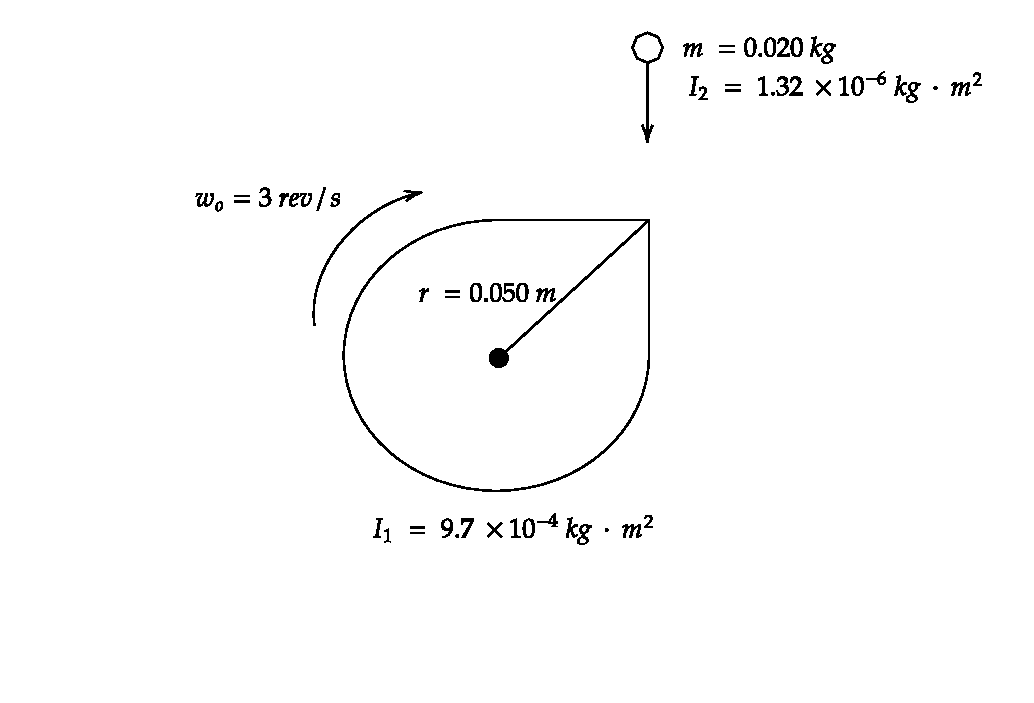
\includegraphics[scale=0.9]{problem5}
	
	\textbf{\underline{Theory}}
	\\
	
	This problem utilizes parallel-axis theorem and the conservation of angular momentum. In order to take advantage of the knowledge that $\vec{L} = \omega I$. We must first find the moment of inertia for the two objects combined using parallel-axis theorem. Then, to get the final answer, we must use the conversation of momentum to solve for the final angular velocity, $\omega_f$.
	\\
	
	\textbf{\underline{Assumptions}}
	\\
	
	For the sake of this problem, we'll need to assume that the collision that ensues is perfectly inelastic, meaning that the two objects will end up sticking together.
	\\
	
	\textbf{\underline{Solution}}
	\\
	
	First, I found the initial momentum.
	
	\[
	\begin{split}
		\vec{L} &= \omega I_1
		\\
		&= (3.0 \unit{rad/s})(9.7 \times 10^{-4} \unit{kg \cdot m})
		\\
		&= 2.91 \times 10^{-3}
	\end{split}
	\]
	
	Next, I found that total inertia of the total mass using parallel-axis theorem.
	
	\[
	\begin{split}
		I_s &= I_2 + mr^2
		\\
		&= 1.32 \times 10^{-6} \unit{kg \cdot m^2} + (0.02 \unit{kg})(0.05 \unit{m})^2
		\\
		&= 5.132 \times 10^{-5} \unit{kg \cdot m^2}
	\end{split}
	\]
	
	Lastly, to find the angular velocity, I used the knowledge that angular momentum was conserved throughout.
	
	\[
	\begin{split}
		\vec{L}_{Before} &= \vec{L}_{After}
		\\
		(3.0 \unit{rev/s})(9.7 \times 10^{-4} \unit{kg \cdot m^2}) &= (9.7 \times 10^{-4} \unit{kg \cdot m^2} + 5.132 \times 10^{-5} \unit{kg \cdot m^2}) \cdot \omega_f
		\\
		\omega_f &= \boxed{2.85 \unit{rev/s}}
	\end{split}
	\]
	
	\textbf{\underline{Conclusion}}
	\\
	
	The angular velocity after the collision is 2.85 rev/s.
	
\end{homeworkProblem}

\pagebreak

\begin{homeworkProblem}
	An odd-shaped object rotates at a speed of 10.0 rev/s. A small 25g mass with moment of inertia $I = 1.5 \times 10^{-6} \unit{kg \cdot m^2}$ is dropped onto the object at a distance of 4.5 cm from its center of mass. The odd-shaped object slows to a speed of 9.0 rev/s. What is the moment of inertia of the oddshaped object?
	\\

\emph{Hints: 1) parallel-axis theorem; 2) angular momentum is constant.}
	\\
	
	\textbf{\underline{Solution}}
	\\
	
	$I_1 = 4.689 \times 10^{-4} \unit{kg \cdot m^2}$
\end{homeworkProblem}


\end{document}
